\documentclass{article}

\usepackage[margin=1in, top=1.5in, bottom=1.5in, columnsep=0.25in]{geometry}
\usepackage[backend=biber, sorting=none]{biblatex}
\usepackage{graphicx}
\usepackage{hyperref}
\usepackage{amsmath}
\usepackage{amssymb}
\usepackage{marvosym}
\usepackage{tikz}
\usepackage{float}
\usepackage[all]{hypcap}
\usepackage[linesnumbered,ruled,vlined]{algorithm2e}
\usepackage{multicol}
\usepackage[framed, numbered]{matlab-prettifier}
\usepackage{courier}

\counterwithin{figure}{section}
\counterwithin{equation}{section}

\addbibresource{references.bib}

\DeclareMathOperator*{\argmin}{arg\,min}

\title{\large Term paper of Control of Communication and Energy Networks \\ 
\LARGE Decentralized PEV Control Based on a Subgradient Method for Mixed-Integer Programming Problems}
\author{Simone Orelli\\1749732\\ \textit{DIAG Department}\\ \textit{University of Rome “La Sapienza”}\\orelli.1749732@studenti.uniroma1.it 
\and Antonio Rapuano\\2044902\\ \textit{DIAG Department}\\ \textit{University of Rome “La Sapienza”}\\rapuano.2044902@studenti.uniroma1.it}
\date{January 2024}


\begin{document}
    \maketitle
    \thispagestyle{empty}
    \begin{multicols}{2}
    \begin{abstract}
    This term paper presents a decentralized approach to the problem of charging a fleet of plug-in electric vehicles (PEVs) in a smart grid, where global and local constraints and objectives are considered together with the model of the power grid by means of a MPC strategy. The representation of the charging problem involves a combination of continuous and integer variables (specifically of Boolean nature). It is formulated as a mixed-integer linear programming (MILP) problem, which is solved using a subgradient method. The proposed approach is compared with a centralized one, which is typically solved by a branch-and-bound algorithm. The results show that the decentralized approach is able to achieve a performance close to the centralized one, while reducing the computational burden, especially for large fleets of vehicles. These findings are supported by means of simulations performed on a test case.
\end{abstract}
    \vfill\null
    \columnbreak

    \tableofcontents

    \newpage
    \setcounter{page}{1}

    \section{Introduction}
\label{sec:introduction}
In recent years, the landscape of transportation has witnessed a transformative shift towards electromobility, reflecting a global commitment to sustainable and environmentally conscious practices. This evolution is propelled by advancements in electric vehicle technology, coupled with an increasing societal awareness of the urgent need to reduce carbon emissions in the transport sector. As the number of electric vehicles increases, the demand for efficient charging strategies becomes paramount to ensure seamless integration into the existing infrastructure.

Consider the following scenario: a fleet of PEVs are connected to a charging station. The charging stations are linked to a central controller, which is responsible for managing the charging process. The controller has to decide the charging rate of each vehicle, taking into account their charging requirements and the power limits of the grid connection. The goal is to minimize the total charging cost tracking the aggregated power reference (i.e. desired value for the total power withdrawn from the grid), while ensuring that the charging process is completed according to the preferences of each driver, expressed in terms of final state of charge and charging time.

Typically, the problem is addressed with Model Predictive Control (MPC) techniques, which are well suited for the management of complex systems with multiple constraints. In such instances, the decentralized approach involves dividing the problem into multiple subproblems, which are collaboratively solved by both the plug-in electric vehicles and the control center. This contrasts with the centralized method where data is collected from PEVs, and a singular computation is performed at the control center, which may become impractical for large-scale systems due to the escalating computational burden associated with an increasing number of variables.

Decentralized approaches have been proposed in the past literature. 
Vujanic et al. (in their work \autocite{VUJANIC2016144}) were among the pioneering researchers exploring scalable PEV charging control solutions by employing decentralized approaches to solve mixed-integer linear problems. Further developments have been proposed by Falsone et al. (in their article \autocite{FALSONE2019141}, for which significant improvements were developed in the recent work \autocite{MANIERI20235919} by Manieri et al.).

The work presented in this document is a thorough review of the developements proposed by Liberati et al. in their article \autocite{10194623}. Their main contributions lie in modeling the charging process of each PEV as a semi-continuous variable and in the inclusion of the additional objective of tracking a desired aggregated power profile. Here, adopting the solution advanced by Falsone et al. in \autocite{FALSONE2019141}, the authors highlight the differences between a centralized and a decentralized approach, both in terms of problem formulation and solution algorithm. The two approaches are finally compared in terms of computational complexity and performance, by means of simulations.

Table \ref{tab:nomenclature} at the end of the document summarizes the nomenclature used.
    \section{Centralized approach}
Consider a set of $m$ PEVs (each with its own specifications) and a MPC prediction horizon of $N = t_f - t_0 + 1$ time steps of duration equal to $T$. The centralized approach consists in computing the optimal charging/discharging schedule for each PEV $p$ at each time step over the prediction horizon, meeting the preferences of the PEV drivers regarding charging time and final state of charge. It is crucial to ensure that the combined power drawn adheres to specified limits and follows a designated pattern, usually calculated to optimize the influence of recharging activities on the electrical grid.
Figure \ref{fig:cen_scheme} shows the block scheme of the centralized approach.
\begin{figure}[H]
    \centering
    \begin{tikzpicture}[node distance=1.5cm]
        \node (grid) [draw, rectangle, text width=2cm, minimum height=2.5cm, align=center, fill=red!20, rounded corners] {Power \\grid};

        \node (pev2) [draw, rectangle, right of=grid, xshift=1.2cm, fill=green!20, rounded corners] {PEV$_2$};
        \node (pev1) [draw, rectangle, above of=pev2, yshift=-0.5cm, fill=green!20, rounded corners] {PEV$_1$};
        \node (pevm) [draw, rectangle, below of=pev2, yshift=0.5cm, fill=green!20, rounded corners] {PEV$_m$};

        \node (demux) [draw, rectangle, minimum width=0.3cm, minimum height=3cm, fill=black, right of=pev2, xshift=-0.2cm] {};

        \node (cc) [draw, rectangle, text width=2cm, minimum height=1.5cm, below of=grid, align=center, yshift=-1cm, fill=blue!20, rounded corners] {Central \\controller};

        \draw [->] ([yshift=1cm]grid.east) -- node[above] {\Lightning} (pev1.west);
        \draw [->] (grid.east) -- node[above] {\Lightning} (pev2.west);
        \draw [->] ([yshift=-1cm]grid.east) -- node[above] {\Lightning} (pevm.west);

        \draw [->] (pev1.east) -- ([yshift=1cm]demux.west);
        \draw [->] (pev2.east) -- (demux.west);
        \draw [->] (pevm.east) -- ([yshift=-1cm]demux.west);

        \draw [draw=white] (pev2) -- node[midway] {...} (pevm);

        \draw [->] (demux.east) -| ([xshift=0.5cm]demux.east) |- node[pos=0.75, above] {$x_p$, $x^{ref}_p$, $F_p$, specs$_p$} (cc.east);
        \draw [->] (cc.west) -| node[pos=0.74, left] {$P_p$}([xshift=-0.5cm]grid.west) -- (grid);
    \end{tikzpicture}
    \caption{Centralized approach block scheme.}
    \label{fig:cen_scheme}
\end{figure}
\subsection{Problem formulation}
\textbf{Goal}: compute the optimal charging/discharging schedule for a set of $m$ PEVs connected to the power grid.
\\\textbf{PEV charging constraints}
\begin{gather}
    -P^{dis,max}_p \leq P_{p,i} \leq P^{ch,max}_p, \quad \forall p,i \label{constr:c1}\\
    P_{p,i} = P^{ch}_{p,i}-P^{dis}_{p,i}, \quad \forall p,i \\
    \delta^{ch}_{p,i} P^{ch,min}_p \leq P^{ch}_{p,i} \leq \delta^{ch}_{p,i} P^{ch,max}_p, \quad \forall p,i \\
    \delta^{dis}_{p,i} P^{dis,min}_p \leq P^{dis}_{p,i} \leq \delta^{dis}_{p,i} P^{dis,max}_p, \quad \forall p,i \\
    \delta^{dis}_{p,i} + \delta^{ch}_{p,i} \leq 1, \quad \forall p,i \label{constr:c5}
\end{gather}
\\\textbf{Aggregated power constraints}
\begin{gather}
    P_i = \sum_{p=1}^m P_{p,i}, \quad \forall i \\
    P_i \leq P^{max}_i, \quad \forall i \label{constr:c7}
\end{gather}
\\\textbf{PEV state of charge evolution}\\
$\forall p,i:$
\begin{align}
    \begin{cases}
        x_{p,i+1} = x_{p,i} + T (\eta^{ch}_p P^{ch}_{p,i} - \frac{1}{\eta^{dis}_p} P^{dis}_{p,i}) \label{constr:c8}\\
        x_{p,t_0} = (x_0)_p
    \end{cases}
\end{align}
\\\textbf{PEV state of charge constraints}
\begin{gather}
    x_{p, F_p} = x^{ref}_p, \quad \forall p \\
    x^{min}_p \leq x_{p,i} \leq x^{max}_p, \quad \forall p,i \label{constr:c10}
\end{gather}
\\\textbf{Objective function to minimize} \\
\begin{align}
    V = \sum_{i=1}^{N} |P_i - P^{ref}_i|
\end{align}
that is possible to linearize, introducing the auxiliary variables $t_i$:
\begin{gather}
    V = \sum_{i=1}^{N} t_i \\
    s.t. \quad -t_i \leq P_i - P^{ref}_i \leq t_i, \quad \forall i \label{constr:c13}
\end{gather}
We then introduce a small perturbation term $\xi_{p,i}, \forall p,i$ in $V$ weighting the power to satisfy Assumption 2.4 of \autocite{VUJANIC2016144}. The final form of the objective function is the following:
\begin{align}
    V = \sum_{i=1}^{N} (t_i + \sum_{p=1}^m P_{p,i} \xi_{p,i}) \label{constr:c14}
\end{align}
\textbf{Charging/discharging schedule} \\
At each iteration of the MPC, the optimal control schedule is computed by solving
\begin{align}
    \begin{bmatrix}
        P^{ch}\\
        P^{dis} 
    \end{bmatrix}
    = \argmin_{P^{ch}, P^{dis}} V
\end{align}
subject to the constraints (\ref{constr:c1})-(\ref{constr:c10}), (\ref{constr:c13}), (\ref{constr:c14}),
\\and using the following notation:
$$P^{ch/dis} \triangleq \begin{bmatrix} 
    P^{ch/dis}_{1,1} & \dots & P^{ch/dis}_{1, N} \\
    \vdots & \ddots & \vdots \\
    P^{ch/dis}_{m,1} & \dots & P^{ch/dis}_{m, N}
\end{bmatrix}$$ 
The charging/discharging schedule of each PEV is:
$$P_p = \begin{bmatrix} P_{p,1} & \dots & P_{p, N} \end{bmatrix}^T = (P^{ch}_{p}-P^{dis}_{p})^T.$$
\subsection{Solution algorithm}
\begin{algorithm}[H]
    \caption{Centralized algorithm.}
    \label{algo:cen}
    \SetKwInOut{Input}{Input}
    \SetKwInOut{Output}{Output}

    \Input{$\Big\{N, T, m, (P^{max}_i, P^{ref}_i)_{i=1}^N, (P^{ch,max}_p,$
    $ P^{ch,min}_p, P^{dis,max}_p, P^{dis,min}_p, \eta^{ch}_p, \eta^{dis}_p,$
    $(x_0)_p, x^{max}_p, x^{min}_p, x^{ref}_p, F_p)_{p=1}^m,$ 
    $(\xi_{p,i})_{i,p=1}^{N,m}\Big\}$}
    \Output{$\Big\{(P^{ch}_{p,i}, P^{dis}_{p,i})_{i,p=1}^{N,m}\Big\}$}
    
    \BlankLine
    \tcp{Solve the optimization problem}
    \vspace*{-0.4cm}
    $$\begin{bmatrix}
            P^{ch}\\
            P^{dis} 
        \end{bmatrix}
        = \argmin_{P^{ch}, P^{dis}} \sum_{i=1}^{N} (t_i + \sum_{p=1}^m P_{p,i} \xi_{p,i}) $$
        $$s.t. \quad (\ref{constr:c1})-(\ref{constr:c10}), (\ref{constr:c13}), (\ref{constr:c14})$$
\end{algorithm}
    \noindent Notice the large quantity of variables and constraints that the central controller has to deal with. 
    \section{Decentralized approach}
The decentralized approach involves the central controller and vehicles collaborating iteratively to find a common solution that meets both local and global constraints and objectives. At each iteration, a tentative charging schedule is computed by each PEV (solving a local optimization problem) and subsequently sent to the main controller. The controller collects the latter and imposes a new set of Lagrange multipliers to the PEVs, corresponding to an updated penalization term for the inner cost functions (see Subsection \ref{sec:dec_problem}). These new multipliers influence the next local tentative charging schedules, and the process iterates until a stop criterion is met. The decentralized approach is summarized in Figure \ref{fig:dec_scheme} (where the iteration process described above is enclosed in the \textit{Fast closed loop}).
\begin{figure}[H]
    \centering
    \begin{tikzpicture}[node distance=1.5cm]
        \node (cc) [draw, rectangle, text width=2cm, minimum height=2.5cm, align=center, fill=blue!20, rounded corners] {Central \\controller};

        \node (pev2) [draw, rectangle, right of=grid, xshift=1.75cm, fill=green!20, rounded corners] {PEV$_2$};
        \node (pev1) [draw, rectangle, above of=pev2, yshift=-0.5cm, fill=green!20, rounded corners] {PEV$_1$};
        \node (pevm) [draw, rectangle, below of=pev2, yshift=0.5cm, fill=green!20, rounded corners] {PEV$_m$};

        \node (demux) [draw, rectangle, minimum width=0.3cm, minimum height=3cm, fill=black, right of=pev2, xshift=-0.2cm] {};

        \node (grid) [draw, rectangle, text width=2cm, minimum height=1.5cm, above of=pev1, align=center, yshift=0.2cm, fill=red!20, rounded corners] {Power\\ grid};

        \draw [->] ([yshift=1cm]cc.east) -- node[above] {$\lambda, \mu, \nu$} (pev1.west);
        \draw [->] (cc.east) -- node[above] {$\lambda, \mu, \nu$} (pev2.west);
        \draw [->] ([yshift=-1cm]cc.east) -- node[above] {$\lambda, \mu, \nu$} (pevm.west);

        \draw [->] (pev1.east) -- ([yshift=1cm]demux.west);
        \draw [->] (pev2.east) -- (demux.west);
        \draw [->] (pevm.east) -- ([yshift=-1cm]demux.west);

        \draw [draw=white] (pev2) -- node[midway] {...} (pevm);

        \draw [->] (demux.east) -| ([xshift=0.5cm, yshift=-2cm]demux.east) -| node[pos=0.245, above] {$P_p, \rho_p$} ([xshift=-0.5cm]cc.west) -- (cc);

        \draw [->] (cc.north) |- node[pos=0.75, above] {$P_p$} (grid.west);

        \draw [->] ([xshift=-0.3cm]grid.south) -- node[pos=0.6, left] {\Lightning} ([xshift=-0.3cm]pev1.north);

        \draw [-] (grid) -- (pev1);
        \draw [->] (pev1) -- node[left] {\Lightning} (pev2);

        \draw [-] ([xshift=0.3cm]grid.south) -- ([xshift=0.3cm]pev1.north);
        \draw [-] ([xshift=0.3cm]pev1.south) -- ([xshift=0.3cm]pev2.north);
        \draw [->] ([xshift=0.3cm]pev2.south) -- node[right] {\Lightning} ([xshift=0.3cm]pevm.north);

        \draw[dashed] ([xshift=-0.3cm, yshift=1cm]current bounding box.west) rectangle ([xshift=0.3cm, yshift=-0.3cm]current bounding box.south east);
        
        \node at ([yshift=-0.32cm]current bounding box.south) {Fast closed loop};
    \end{tikzpicture}
    \caption{Decentralized approach block scheme.}
    \label{fig:dec_scheme}
\end{figure}
\subsection{Problem formulation}
\label{sec:dec_problem}
\textbf{Inner minimization problem} \\
The dual function is obtained by dualizing the coupling constraints (\ref{constr:c7}) and (\ref{constr:c13}) and by imposing $\mu_i +\nu_i \leq 1$,  as in \autocite{10194623}:
\begin{gather*}
    d(\lambda, \mu, \nu) = \sum_{p=1}^m min_{P_p} P_p(\xi_p + \lambda +\mu - \nu) + \\
    - (\mu - \nu)P^{ref} - \lambda(P^{max} - \rho)
\end{gather*}
subject to the constraints (\ref{constr:c1})-(\ref{constr:c5}), (\ref{constr:c8})-(\ref{constr:c10}).

The inner minimization problem is decomposed in $m$ decoupled subproblems, one for each PEV $p$, solvable in parallel. The optimal solution of the $p$-th subproblem is:
\begin{gather}
    P_p = \argmin_{P_p} P_p(\xi_p + \mu - \nu + \lambda) \label{eq:optimalPp}
\end{gather} $$s.t. \quad (\ref{constr:c1})-(\ref{constr:c5}), (\ref{constr:c8})-(\ref{constr:c10})$$ \\
\textbf{Outer minimization problem} \\
Once the optimal solution of the inner minimization problem is found at the level of each PEV, the $m$ tentative charging schedules are shared to the central controller. The controller then updates the Lagrange multipliers accordingly to some decreasing step size $\alpha(k)$, chosen so as to satisfy the following conditions:
\begin{gather*}
    \lim_{k \to \infty} \alpha(k) = 0, \\
    \sum_{k=1}^\infty \alpha(k) = \infty, \\
    \sum_{k=1}^{\infty} \alpha(k)^2 < \infty,
\end{gather*}
as requested in the standard dual subgradient method. This process is repeated until the dual subgradient method achieves asymptotic convergence.

\subsection{Solution algorithm}
Algorithm \ref{algo:dec} is a variant of the dual subgradient method, where two are the main steps:
\begin{itemize}
    \item computation of the subgradient of the dual function (line 5);
    \item update of the Lagrange multipliers with $\alpha$ as step size (lines 10-13).
\end{itemize}
The maximum and minimum operations are to be intended component-wise.
Notice the decreased number of inputs with respect to the centralized algorithm.

\begin{algorithm}[H]
    \label{algo:dec}
    \caption{Decentralized algorithm.}
    \SetKwInOut{Input}{Input}
    \SetKwInOut{Output}{Output}

    \Input{$\Big\{N, T, m, (P^{max}_i, P^{ref}_i)_{i=1}^N, (\xi_{p,i})_{i,p=1}^{N,m}\Big\}$}
    \Output{$\Big\{(P^{ch}_{p,i}, P^{dis}_{p,i})_{i,p=1}^{N,m}\Big\}$}

    \BlankLine
    \tcp{Initialize the variables}
    $k=0$, $\lambda(k)=0$, $\mu(k)=0$, $\nu(k)=0$ \\
    $\overline{s}_p = -\infty$, $\underline{s}_p = +\infty$ for $p=1,\dots,m$
    
    \BlankLine
    \tcp{Outer optimization problem}
    \Repeat{termination condition is met}{
        \For{$p=1,...,m$}{
            \tcp{Inner optimization problem}
            \vspace*{-0.4cm}
            \begin{gather*}
                P_{p}(k+1) = \argmin_{P_p} \Big[P_p(k)\Big(\xi_p + \lambda(k)+ \\
                + \mu(k)- \nu(k)\Big)\Big] \\
                s.t. \quad (\ref{constr:c1})-(\ref{constr:c5}), (\ref{constr:c8})-(\ref{constr:c10})
            \end{gather*}

            $\overline{s}_p = \max\{\overline{s}_p, P_p(k+1)\}$ \\
            $\underline{s}_p = \min\{\underline{s}_p, P_p(k+1)\}$ \\
            $\rho_p(k+1) = \overline{s}_p - \underline{s}_p$
        }
        \BlankLine
        \tcp{Update the multipliers}
        $\rho(k+1) = N \max\Big\{\Big(\rho_p(k+1)\Big)_{p=1}^m\Big\}$ \\
        $\lambda (k+1) =$ $max\Big\{0,\lambda (k) + a(k)\Big(\sum^{m}_{p=1} P_p(k+ 1) - P^{max} + \rho\Big)\Big\}$\;
        $\mu (k+1) = max\Big\{0,\mu (k) + a(k)\Big(\sum^{m}_{p=1} P_p(k+ 1) - P^{ref}\Big)\Big\}$\;
        $\nu (k+1) = max\Big\{0,\nu (k) - a(k)\Big(\sum^{m}_{p=1} P_p(k+ 1) - P^{ref} \Big)\Big\}$\;
        $k++$
    }
\end{algorithm}
    \section{Simulations}
The simulations have been performed adopting the parameters in Table \ref{tab:sim_param} using \textit{MATLAB R2023b}. The \textit{Optimization Toolbox} and the \textit{Global Optimization Toolbox} provided the utilities to solve the MILP problems (in particular, the \textit{intlinprog} solver), while \textit{Parallel Computing Toolbox} has been exploited to take avantage of the modularity of the decentralized problem in order to speed up the computation employing multiple CPU cores, each effectively corrisponding to a cluster of PEVs. The code is shown in Appendix \ref{sec:matlab}.
\begin{table}[H]
    \centering
    \begin{tabular}{|c|c|}
        \hline
        Symbol & Value \\
        \hline
        $m$ & $500$ \\
        $N = F_p$ & $24$ \\
        $T$ [min] & $20$ \\
        $P^{max}$ [kW] & $\{500, 200, 500\}$ \\
        $P^{ref}$ [kW] & $290$ \\
        $P^{ch,max}_p$ [kW] & $3.3$ \\
        $x^{max}_p$ [kWh] & $[8, 16]$ \\
        $x^{min}_p$ [kWh] & $1$ \\
        $(x_0)_p$ [kWh] & $[0.2, 0.5] \cdot x^{max}_p$ \\
        $x^{ref}_p$ [kWh] & $[0.55, 0.8] \cdot x^{max}_p$ \\
        $\eta^{ch}_p$ & $[0.925, 0.985]$ \\
        $\xi_p$ & $[0, 0.3]$ \\
        \hline
    \end{tabular}
    \caption{Simulation parameters.}
    \label{tab:sim_param}
\end{table}

\subsection{Centralized approach}
Figure \ref{fig:cen_power} shows the power profile of the PEVs in the centralized approach. The aggregated power tracks almost perfectly the reference value, without ever exceeding the constraint on the maximum power.
\begin{figure}[H]
    \centering
    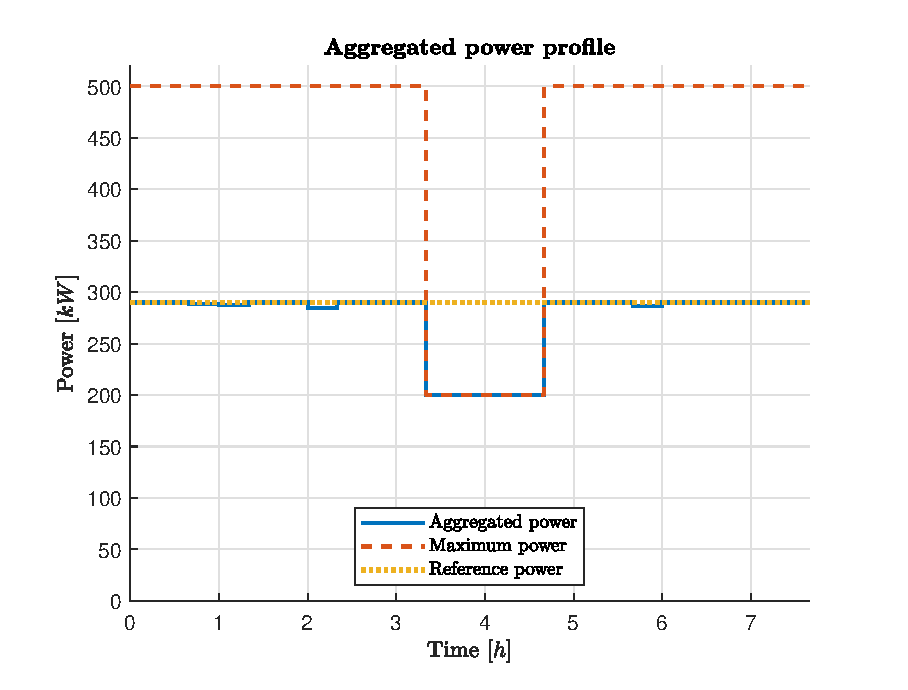
\includegraphics[width=\columnwidth]{figures/images/cen_power.eps}
    \caption{Aggregated power profile of the PEVs in the centralized case.}
    \label{fig:cen_power}
\end{figure}

The state of charge evolution of a random batch of 10 PEVs can be seen in Figure \ref{fig:cen_state}. The state of charge is kept within the limits and the final values reflect the desired ones.
\begin{figure}[H]
    \centering
    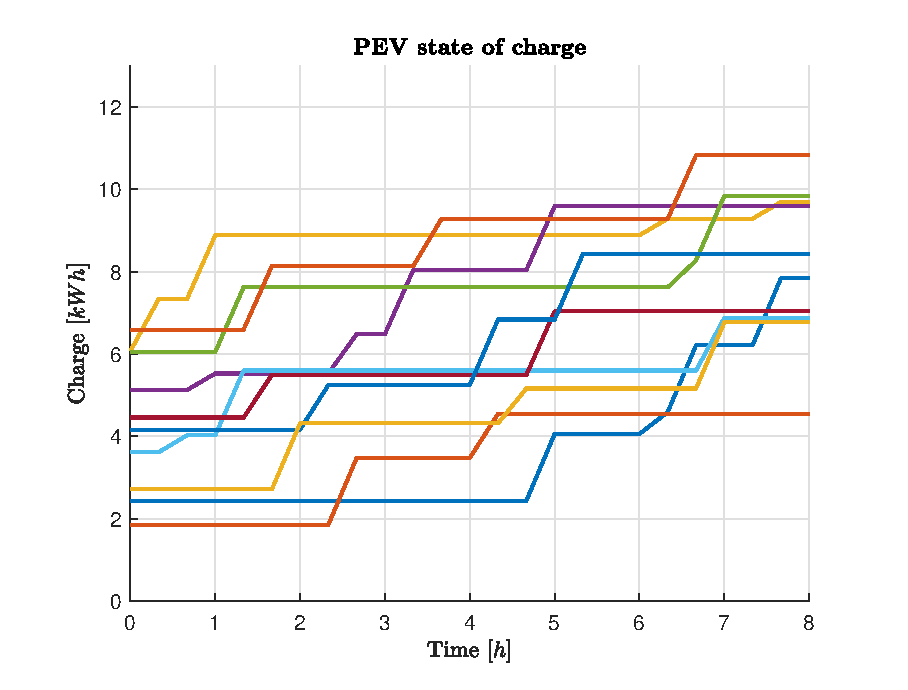
\includegraphics[width=\columnwidth]{figures/images/cen_state.eps}
    \caption{State of charge evolution of the PEVs in the centralized case.}
    \label{fig:cen_state}
\end{figure}

Finding the optimal solution of the centralized problem takes about $414.3\,s \simeq 7\,min $. This is typically not acceptable in a real-world scenario, where the optimization problem should be solved in a significantly shorter time than the duration of the sampling step.
\subsection{Decentralized approach}
The simulation is carried out setting the step size $\alpha(k) = \frac{0.001}{k+1}$. The termination condition is met when the aggregated power profile is under the threshold $P^{max}_i$ and is within $30 kW$ of the minimum between $P^{max}_i$ and the reference $P^{ref}_i$.

Figure \ref{fig:dec_stop_criterion} shows the amount of maximum violation of the global constraint and the maximum deviation between the solution and the reference (regarding the maximum aggregated power). In particular, for small values of k (i.e., the initial iterations of the algorithm) the PEVs try to greedily impose a (globally unfeasible) charging schedule. As the iterations proceed, the central controller modifies the Lagrange multipliers $\lambda$, $\mu$, $\nu$ in order to force the convergence to a feasible solution, which is reached after $17$ iterations. As a matter of fact, that is when the termination condition is met.

The aggregated power profile solution is shown in Figure \ref{fig:dec_power}. Notice that it always satifies the global constraint, even though it is not as faithful to the reference as the centralized solution. This is due to the fact that the PEVs do not have access to the global information.


\begin{figure}[H]
    \centering
    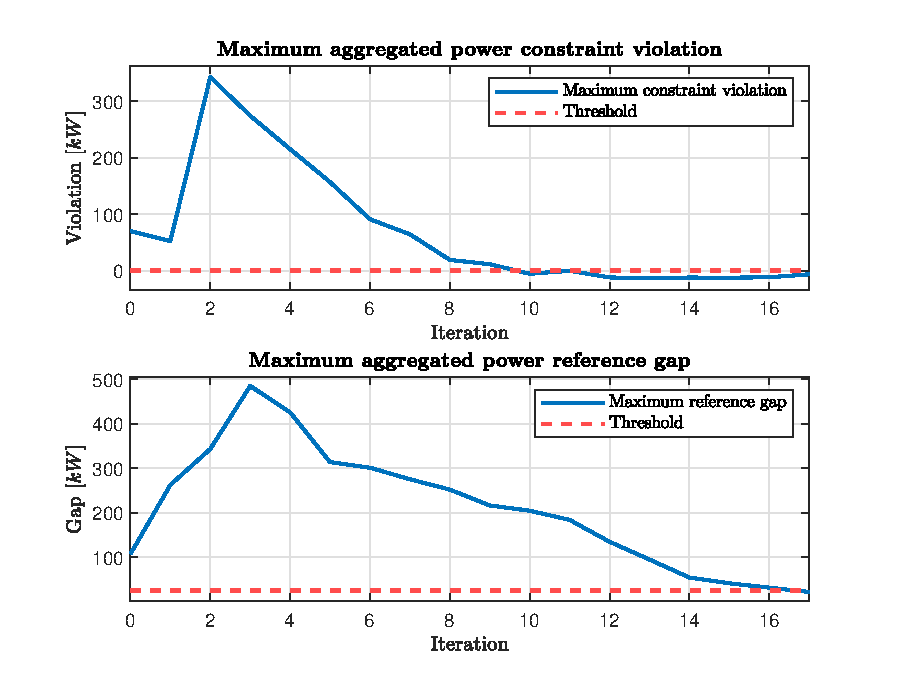
\includegraphics[width=\columnwidth]{figures/images/stop_criterion.eps}
    \caption{Maximum global constraint violation and maximum deviation from the adjusted reference per iteration of the decentralized algorithm.}
    \label{fig:dec_stop_criterion}
\end{figure}

\begin{figure}[H]
    \centering
    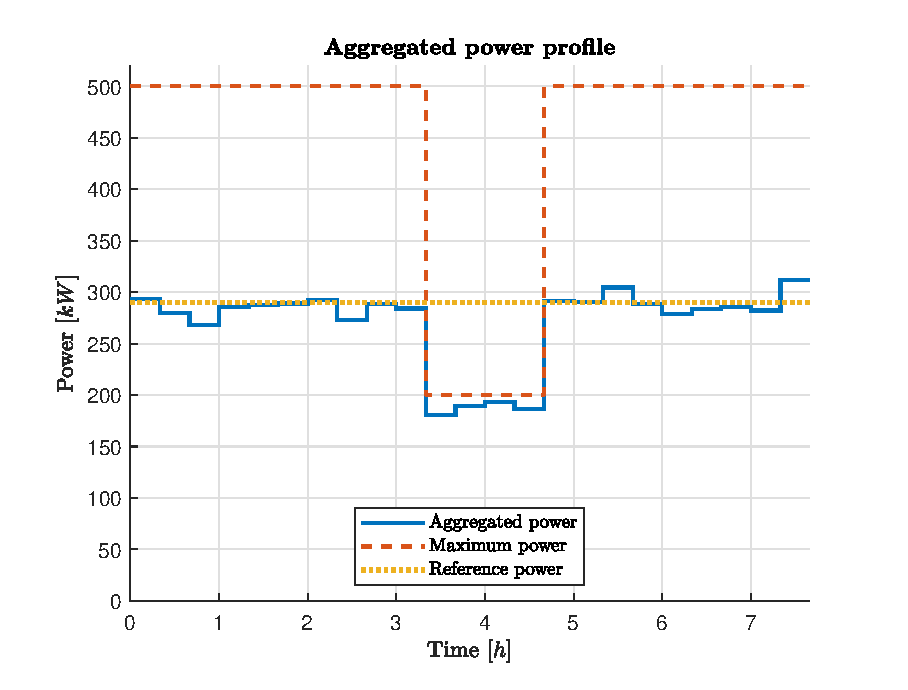
\includegraphics[width=\columnwidth]{figures/images/dec_power.eps}
    \caption{Aggregated power profile of the PEVs in the decentralized case.}
    \label{fig:dec_power}
\end{figure}

\begin{figure}[H]
    \centering
    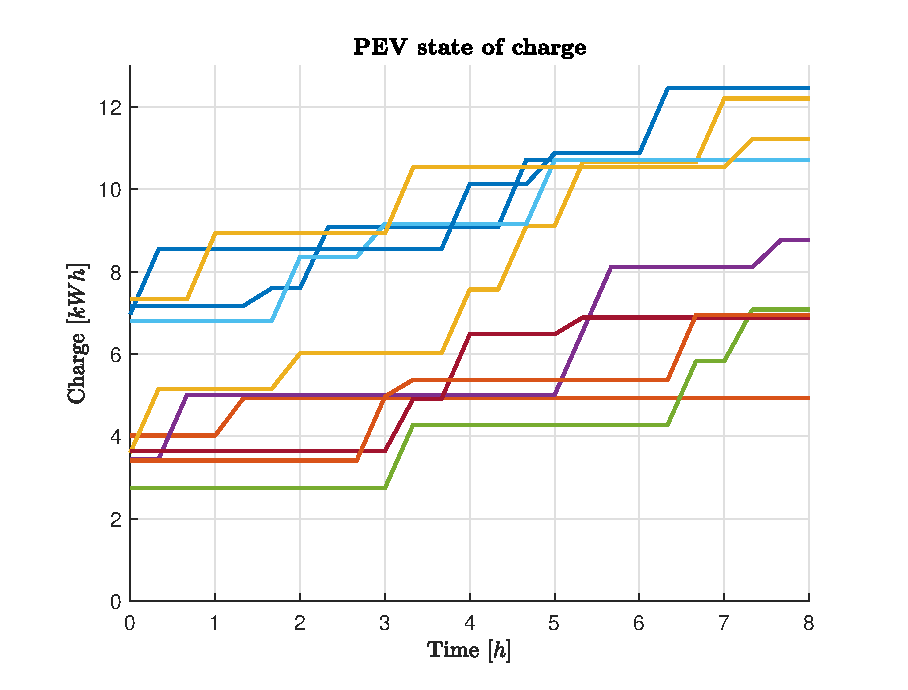
\includegraphics[width=\columnwidth]{figures/images/dec_state.eps}
    \caption{State of charge evolution of the PEVs in the decentralized case.}
    \label{fig:dec_state}
\end{figure}


Figure \ref{fig:dec_state} displays the state of charge of a random batch of 10 PEVs. As in the centralized case, the charging process is carried out correctly.

The evolution of $||\rho_p||_2$ can be analyzed in Figure \ref{fig:dec_rho} accordingly to line 9 of Algorithm \ref{algo:dec}. The increase of the magnitude of $\rho_p$ goes hand in hand with the approach to the globally feasible optimal solution (compare with Figure \ref{fig:dec_stop_criterion}).

Finally, in Figure \ref{fig:dec_multipliers} the consequent progression of the multipliers is displayed. Iteration after iteration, they are updated according to lines 11-13 of Algorithm \ref{algo:dec}, and they play a crucial role in the computation of the solutions of the inner optimization problems (line 5). In fact, since in the first iterations the global constraints are violated, the multipliers mutate in order to force the convergence to a feasible solution. 
\begin{figure}[H]
    \centering
    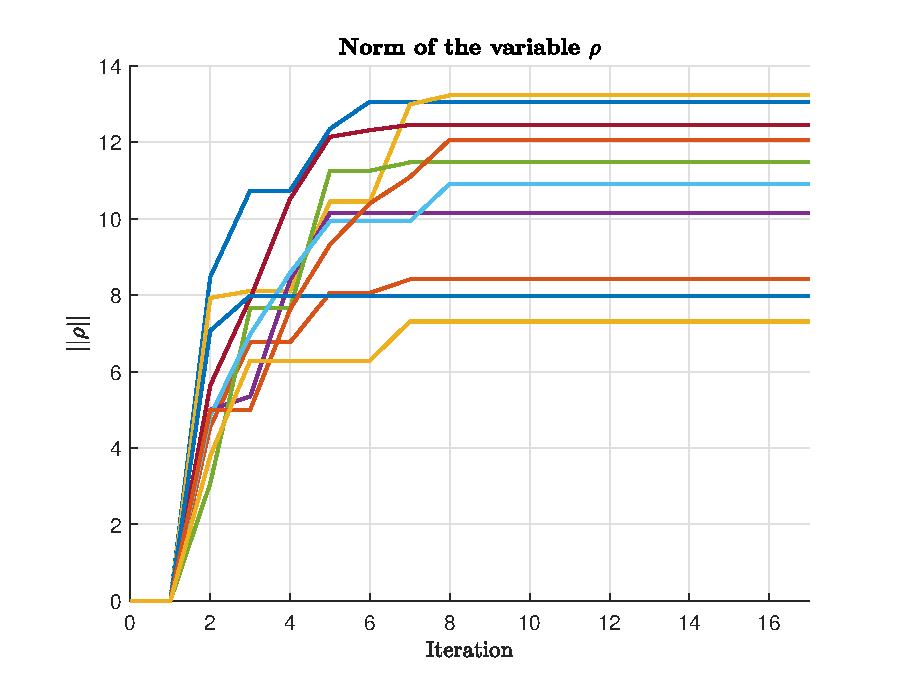
\includegraphics[width=\columnwidth]{figures/images/rho.eps}
    \caption{Norm of $\rho$ for a random batch of $10$ PEVs per iteration of the decentralized algorithm.}
    \label{fig:dec_rho}
\end{figure}


In terms of computational burden, there is a significant improvement with respect to the centralized approach. By averaging the time that each PEV takes to solve the inner optimization problem, we get $0.159\,s$. Hence, to carry out 17 iterations, the algorithm takes about $2.7\,s$.
\end{multicols}
\begin{figure}[H]
    \center
    \begin{minipage}{5.4cm}
        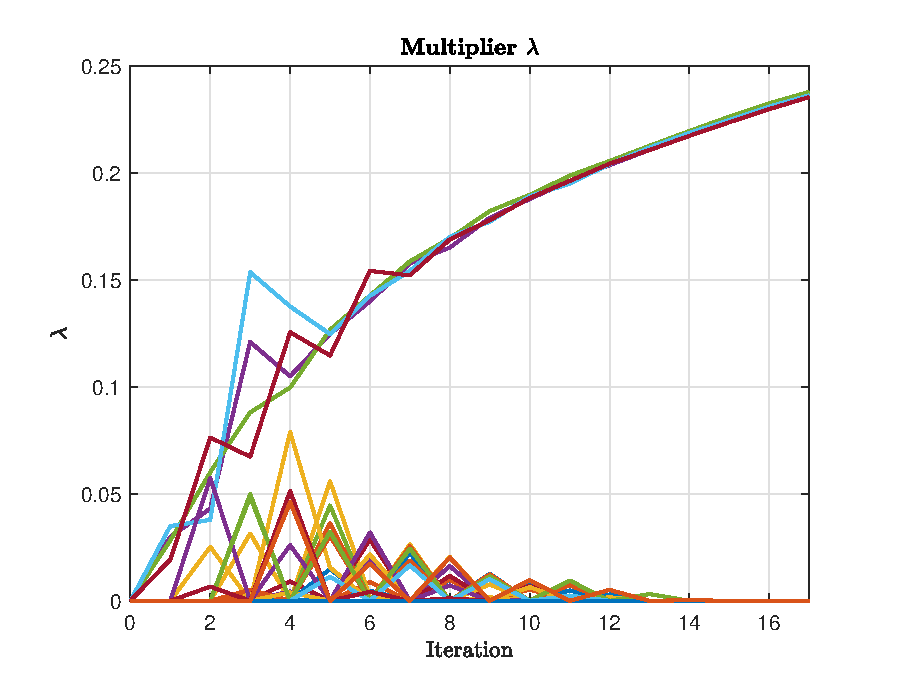
\includegraphics[width=\columnwidth]{figures/images/lambda.eps}
    \end{minipage}
    \begin{minipage}{5.4cm}
        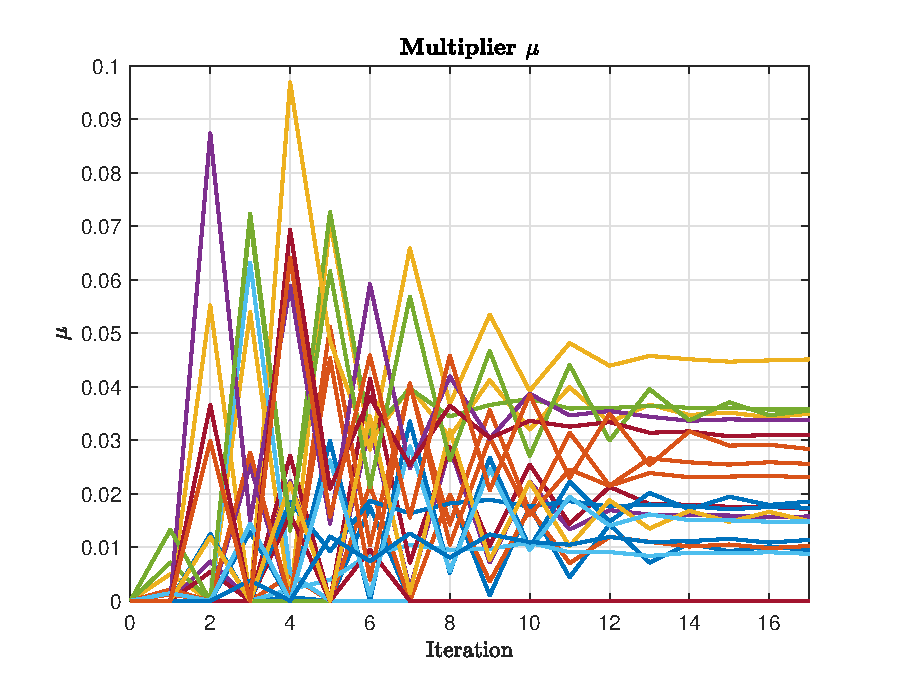
\includegraphics[width=\columnwidth]{figures/images/mu.eps}
    \end{minipage}
    \begin{minipage}{5.4cm}
        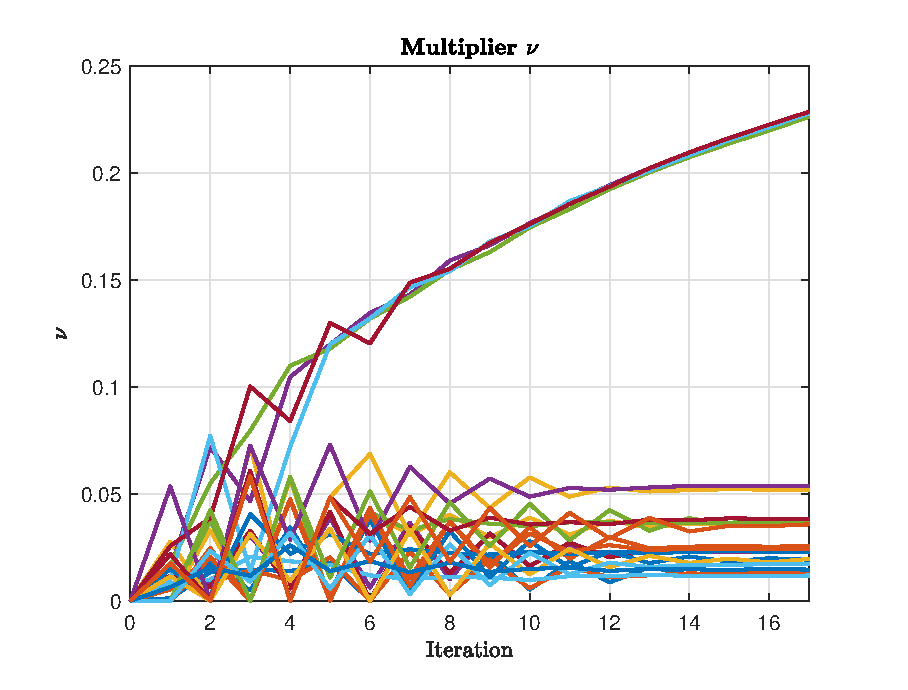
\includegraphics[width=\columnwidth]{figures/images/nu.eps}
    \end{minipage}
    \caption{Evolution of the Lagrange multipliers per iteration of the decentralized algorithm.}
    \label{fig:dec_multipliers}
\end{figure}
\begin{multicols}{2}
    \section{Conclusions}
In the present document, two different approaches to the PEV charging problem have been presented. The first one is a centralized approach, where the problem is solved by a single entity that has access to all the information about the system. The second one is a decentralized approach, where the problem is solved by a set of agents that have access only to local information, supervised by a central entity. The analysis of the two approaches has been carried out both in qualitative (level of performance) and quantitative (computational burden) terms.

The centralized algorithm manages to find a solution that satisfies the requests of the PEV owners, while keeping the power flow in the network within the limits and almost perfectly equal to the reference. However, it is important to highlight that its computational load is very high, and is not suitable for real-time applications. In fact, the computational time is of the order of minutes, and it is not possible to reduce it significantly without losing the optimality of the solution. Moreover, this controller requires a lot of sensitive information about the PEVs, such as the arrival and departure times, the battery capacity and the required energy. 

On the other hand, the decentralized algorithm identifies a feasible solution that is sufficiently close to the centralized one in a noticeably shorter time. Besides, the central unit does not require any sensitive information about the PEVs, as all the necessary data is coded in the form of the local tentative power schedules.
    \vfill\null
    \columnbreak

    \appendix
    \end{multicols}
\section{MATLAB implementation}
\label{sec:matlab}
\subsection{Centralized approach}
\textbf{Centralized MPC class}
\lstinputlisting[style=Matlab-editor, basicstyle=\footnotesize\ttfamily]{scripts/CenMpc.m}
\vspace*{0.1cm}
\textbf{Main script}
\lstinputlisting[style=Matlab-editor, basicstyle=\footnotesize\ttfamily]{scripts/centralized_PEV_charging_simple.m}
\subsection{Decentralized approach}
\textbf{PEV MPC class}
\lstinputlisting[style=Matlab-editor, basicstyle=\footnotesize\ttfamily]{scripts/PevMpc.m}
\vspace*{0.1cm}
\textbf{Main script}
\lstinputlisting[style=Matlab-editor, basicstyle=\footnotesize\ttfamily]{scripts/decentralized_PEV_charging_simple.m}

    \begin{table}[H]
    \centering
    \begin{tabular}{|c|p{0.7\columnwidth}|}
        \hline
        Symbol & Explanation \\
        \hline
        \(m\) & Number of PEVs. \\
        \(N\) & MPC prediction horizon. \\
        \(t_f\) & Final instant of the problem. \\
        \(t_0\) & Initial instant of the problem. \\
        \(T\) & Sampling time. \\
        \(p\) & Index to denote a generic PEV. \\
        \(i\) & Index to denote a generic time. \\
        \(P_{p,i}\) & Charging/discharging power of PEV $p$ at time $i$. \\
        \(P^{ch}_{p,i}\) & Charging power of PEV $p$ at time $i$. \\
        \(P^{dis}_{p,i}\) & Discharging power of PEV $p$ at time $i$. \\
        \(P^{ch,min}_p\) & Minimum charging power of PEV $p$. \\
        \(P^{ch,max}_p\) & Maximum charging power of PEV $p$. \\
        \(P^{dis,min}_p\) & Minimum discharging power of PEV $p$. \\
        \(P^{dis,max}_p\) & Maximum discharging power of PEV $p$. \\
        \(\delta^{ch}_{p,i}\) & $\in \{0, 1\}.$ 1 if PEV $p$ is charging at time $i$, 0 otherwise. \\
        \(\delta^{dis}_{p,i}\) & $\in \{0, 1\}.$ 1 if PEV $p$ is discharging at time $i$, 0 otherwise. \\
        \(P_i\) & Aggregated power at time $i$. \\
        \(P^{max}_i\) & Maximum aggregated power at time $i$. \\
        \(x_{p,i}\) & State of charge of PEV $p$ at time $i$. \\
        \((x_0)_p\) & Initial state of charge of PEV $p$. \\
        \(\eta^{ch}_p\) & $\in (0, 1).$ Charging efficiency of PEV $p$. \\
        \(\eta^{dis}_p\) & $\in (0, 1).$ Discharging efficiency of PEV $p$. \\
        \(F_p\) & Desired charging end instant of PEV $p$. \\
        \(x^{ref}_p\) & $= x_{p, F_p}.$ Desired final state of charge of PEV $p$. \\
        \(x^{max_p}\) & Maximum state of charge of PEV $p$. \\
        \(x^{min_p}\) & Minimum state of charge of PEV $p$. \\
        \(P^{ref}_i\) & Reference aggregated power at time $i$. \\
        \(V\) & Objective function to minimize. \\
        \(t_i\) & Auxiliary variable to linearize the objective function. \\
        \(\xi_{p,i}\) & Perturbation term in the objective function. \\
        \(\lambda, \mu, \nu\) & Lagrange multipliers. \\
        \(\overline{s}_p\, \underline{s}_p\) & Auxiliary variables to compute the virtual price term. \\
        \(\rho\) & Virtual price term \\
        \hline
    \end{tabular}
    \caption{Nomenclature used in the term paper.}
    \label{tab:nomenclature}
\end{table}

    \printbibliography
\end{document}